

\tikzset{every picture/.style={line width=0.75pt}} %set default line width to 0.75pt        

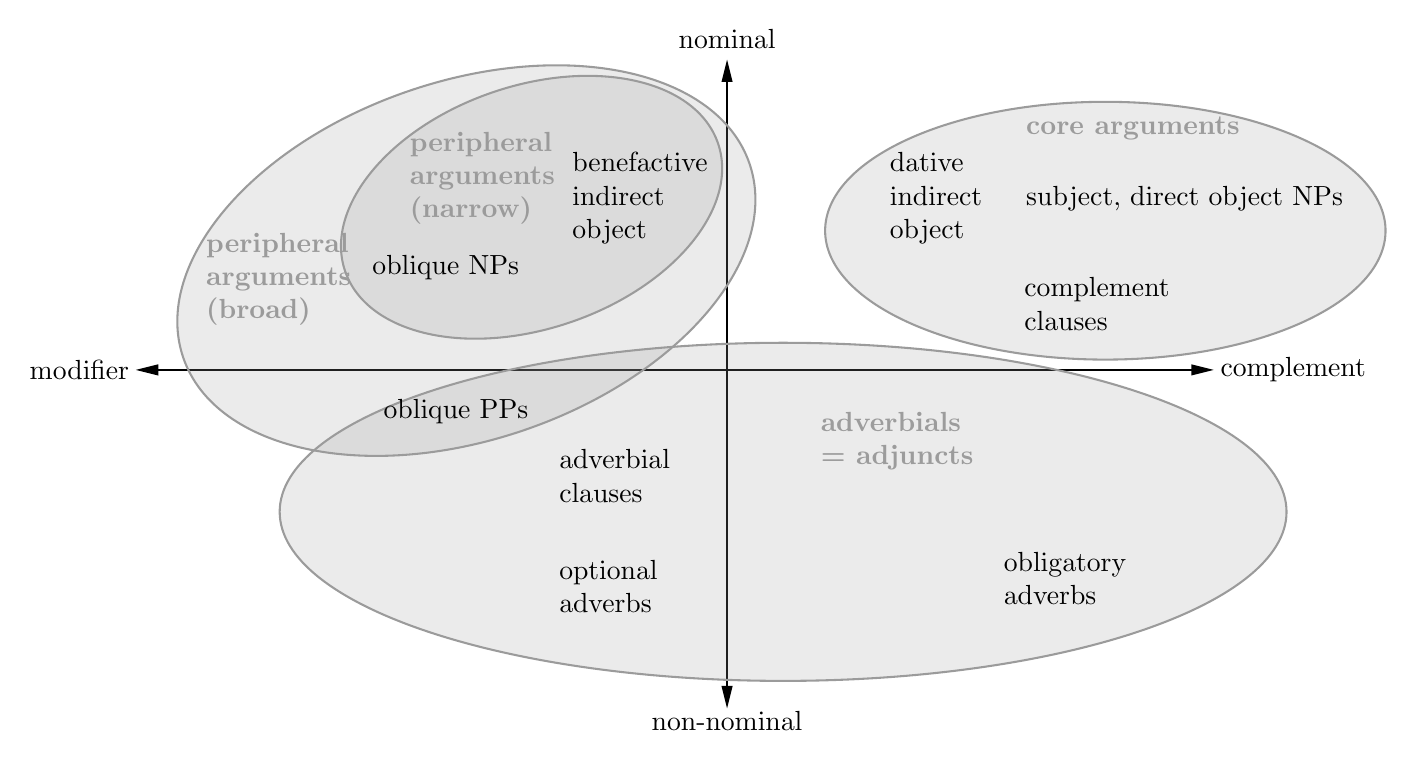
\begin{tikzpicture}[x=0.75pt,y=0.75pt,yscale=-0.9,xscale=0.9]
%uncomment if require: \path (0,401); %set diagram left start at 0, and has height of 401

%Straight Lines [id:da009476237276789146] 
\draw    (98,198) -- (671,198) ;
\draw [shift={(673,198)}, rotate = 180] [fill={rgb, 255:red, 0; green, 0; blue, 0 }  ][line width=0.08]  [draw opacity=0] (12,-3) -- (0,0) -- (12,3) -- cycle    ;
\draw [shift={(96,198)}, rotate = 0] [fill={rgb, 255:red, 0; green, 0; blue, 0 }  ][line width=0.08]  [draw opacity=0] (12,-3) -- (0,0) -- (12,3) -- cycle    ;
%Straight Lines [id:da7773022804601077] 
\draw    (412.5,377.14) -- (412.5,33.86) ;
\draw [shift={(412.5,31.86)}, rotate = 90] [fill={rgb, 255:red, 0; green, 0; blue, 0 }  ][line width=0.08]  [draw opacity=0] (12,-3) -- (0,0) -- (12,3) -- cycle    ;
\draw [shift={(412.5,379.14)}, rotate = 270] [fill={rgb, 255:red, 0; green, 0; blue, 0 }  ][line width=0.08]  [draw opacity=0] (12,-3) -- (0,0) -- (12,3) -- cycle    ;
%Shape: Ellipse [id:dp6612766652403343] 
\draw  [color={rgb, 255:red, 155; green, 155; blue, 155 }  ,draw opacity=1 ][fill={rgb, 255:red, 155; green, 155; blue, 155 }  ,fill opacity=0.2 ] (465,123.48) .. controls (465,85.37) and (532.16,54.48) .. (615,54.48) .. controls (697.84,54.48) and (765,85.37) .. (765,123.48) .. controls (765,161.59) and (697.84,192.48) .. (615,192.48) .. controls (532.16,192.48) and (465,161.59) .. (465,123.48) -- cycle ;
%Shape: Ellipse [id:dp35746311023681887] 
\draw  [color={rgb, 255:red, 155; green, 155; blue, 155 }  ,draw opacity=1 ][fill={rgb, 255:red, 155; green, 155; blue, 155 }  ,fill opacity=0.2 ] (208.04,145.17) .. controls (196.4,111.22) and (231.65,68.38) .. (286.77,49.48) .. controls (341.89,30.57) and (396.01,42.76) .. (407.65,76.71) .. controls (419.29,110.65) and (384.04,153.49) .. (328.92,172.4) .. controls (273.8,191.3) and (219.68,179.11) .. (208.04,145.17) -- cycle ;
%Shape: Ellipse [id:dp7325522804450764] 
\draw  [color={rgb, 255:red, 155; green, 155; blue, 155 }  ,draw opacity=1 ][fill={rgb, 255:red, 155; green, 155; blue, 155 }  ,fill opacity=0.2 ] (121.39,191.46) .. controls (104.22,141.37) and (158.14,77.5) .. (241.84,48.79) .. controls (325.54,20.09) and (407.32,37.42) .. (424.49,87.51) .. controls (441.67,137.6) and (387.75,201.47) .. (304.05,230.18) .. controls (220.35,258.88) and (138.57,241.55) .. (121.39,191.46) -- cycle ;
%Shape: Ellipse [id:dp17093026002033596] 
\draw  [color={rgb, 255:red, 155; green, 155; blue, 155 }  ,draw opacity=1 ][fill={rgb, 255:red, 155; green, 155; blue, 155 }  ,fill opacity=0.2 ] (173,273.98) .. controls (173,224) and (293.66,183.48) .. (442.5,183.48) .. controls (591.34,183.48) and (712,224) .. (712,273.98) .. controls (712,323.96) and (591.34,364.48) .. (442.5,364.48) .. controls (293.66,364.48) and (173,323.96) .. (173,273.98) -- cycle ;

% Text Node
\draw (571,98) node [anchor=north west][inner sep=0.75pt]   [align=left] {subject, direct object NPs};
% Text Node
\draw (675,198) node [anchor=west] [inner sep=0.75pt]   [align=left] {complement};
% Text Node
\draw (94,198) node [anchor=east] [inner sep=0.75pt]   [align=left] {modifier};
% Text Node
\draw (412.5,27.86) node [anchor=south] [inner sep=0.75pt]   [align=left] {nominal};
% Text Node
\draw (412.5,379.14) node [anchor=north] [inner sep=0.75pt]   [align=left] {non-nominal};
% Text Node
\draw (498,80) node [anchor=north west][inner sep=0.75pt]   [align=left] {dative \\indirect \\object};
% Text Node
\draw (570,147) node [anchor=north west][inner sep=0.75pt]   [align=left] {complement \\clauses};
% Text Node
\draw (328,80) node [anchor=north west][inner sep=0.75pt]   [align=left] {benefactive \\indirect \\object};
% Text Node
\draw (221,135) node [anchor=north west][inner sep=0.75pt]   [align=left] {oblique NPs};
% Text Node
\draw (227,212) node [anchor=north west][inner sep=0.75pt]   [align=left] {oblique PPs};
% Text Node
\draw (559,294) node [anchor=north west][inner sep=0.75pt]   [align=left] {obligatory\\adverbs};
% Text Node
\draw (321,298) node [anchor=north west][inner sep=0.75pt]   [align=left] {optional\\adverbs};
% Text Node
\draw (321,239) node [anchor=north west][inner sep=0.75pt]   [align=left] {adverbial \\clauses};
% Text Node
\draw (571,61) node [anchor=north west][inner sep=0.75pt]  [color={rgb, 255:red, 155; green, 155; blue, 155 }  ,opacity=1 ] [align=left] {\textbf{\textcolor[rgb]{0.61,0.61,0.61}{core arguments}}};
% Text Node
\draw (241,69) node [anchor=north west][inner sep=0.75pt]  [color={rgb, 255:red, 155; green, 155; blue, 155 }  ,opacity=1 ] [align=left] {\textbf{peripheral}\\\textbf{arguments}\\\textbf{(narrow)}};
% Text Node
\draw (132,123) node [anchor=north west][inner sep=0.75pt]  [color={rgb, 255:red, 155; green, 155; blue, 155 }  ,opacity=1 ] [align=left] {\textbf{peripheral }\\\textbf{arguments}\\\textbf{(broad)}};
% Text Node
\draw (461,219) node [anchor=north west][inner sep=0.75pt]   [align=left] {\textcolor[rgb]{0.61,0.61,0.61}{\textbf{adverbials}}\\\textbf{\textcolor[rgb]{0.61,0.61,0.61}{= adjuncts}}};


\end{tikzpicture}
